%%%%%%%%%%%%%%%%%%%%%%%%%%%%%%%%%%%%%%%%%%%%%%%%%%%%%%%%%%%%%%%%%%%%%%
%
% 都市システム工学科 特別研究概要テンプレート(2015 年度版)
%
%%%%%%%%%%%%%%%%%%%%%%%%%%%%%%%%%%%%%%%%%%%%%%%%%%%%%%%%%%%%%%%%%%%%%%

\documentclass[a4paper,10pt]{jarticle}
\usepackage[dvipdfmx]{graphicx}
\usepackage{amsmath}
\usepackage{here}
\usepackage{comment}
\usepackage{indentfirst}
\usepackage{slashbox}
\textwidth      18.0cm
\textheight     27.0cm
\oddsidemargin  -1.0cm
\evensidemargin -1.0cm
\topmargin      -2.3cm
\footskip        0.5cm
\columnsep       2.5zw

\renewcommand{\baselinestretch}{0.95}
\pagestyle{empty}

\makeatletter
\def\section{\@startsection {section}{1}{\z@}{-3.5ex plus -1ex minus 
 -.2ex}{2.3ex plus .2ex}{\normalsize \bf}}
\def\subsection{\@startsection {subsection}{1}{\z@}{-3.5ex plus -1ex minus 
 -.2ex}{2.3ex plus .2ex}{\normalsize \bf}}
\makeatother

\begin{document}
\twocolumn[
\begin{center}
 \vspace{-2mm}
 \begin{large}
  {\bf 設置者の稼働時間を考慮した止水板最適設置順序の算出}\\

 \end{large}
 \vspace{-2mm}
\end{center}
 {\bf システム最適化研究室}
 \hfill {\bf 都 14-86 竹内 美紗}
 \vspace{5mm}
] %End of twocolumn

%% vspace のあとの寸法は,出来上がりイメージを見て適宜修正すること

%%%%%%%%%%%%%%%%%%%%%%%%%%%%%%%%%%%%%%%%%%%%%%%%%%%%%%%%%%%%%%%%%%%%%%
\vspace{-8mm}
\section{はじめに}
\vspace{-2.5mm}
%%%%%%%%%%%%%%%%%%%%%%%%%%%%%%%%%%%%%%%%%%%%%%%%%%%%%%%%%%%%%%%%%%%%%%

近年,我が国では都市部において局地的・集中的な豪雨による水害が発生して
%
%いる.特に,1 時間に 100 mm を超える局地的な豪雨がしばしば観測されるよう
%になって
%
おり,地下空間における短時間集中型の豪雨への対策が求められている.
%
そのような状況を踏まえ,先行研究 \cite{水工学論文集2,水工学論文集1} では,
梅田の地下街を対象として,下水道施設を考慮した内水氾濫解析が行われた.そ
の結果,地下空間に流入する出入口の場所,流入順序,流入時間,流入量を推定
することができ,事前に止水活動や避難活動が可能であることが示された.

さらに \cite{武田さん卒論} では,
%地下空間の浸水対策として,
ホワイティうめだを対象とした内水氾濫シュミレーションが行われた.地下街の
管理者は十分な対策が取れず,人員を十分確保できないリスクや,止水板の設置
途中で浸水が始める可能性を考慮して止水板設置順序や設置タイミングなどが検
討された.

一方,馬谷 \cite{馬谷さん卒論} は,この問題を最適化問題として定式化し,最
適化ソルバを用いて解くことで最適な設置順序を算出した.ここでは,各出入り
口から水が流入する時間の合計を最小化することを目的としていた.
%この定式化は汎用的なものではあったが,
しかし,計算条件にいくつか問題点が見られる.
%
例えば \cite{馬谷さん卒論} では設置チームの稼働時間に制限が設けられていな
かった.しかし,止水板の設置は重労働であるため,設置チームの稼働時間に上
限があると考えるのが自然である.また, \cite{馬谷さん卒論} では梅田地下街
全域を対象として最適な設置順序を算出していたが,梅田地下街には複数の管理
主体が存在し,豪雨時にはそれぞれの管理施設に存在する流入する可能性のある
出入り口に止水板を設置することになるはずである.

そこで本研究では,管理主体を考慮しつつ,設置チームの稼働時間に上限を設け
た場合の最適な設置順序を算出する.また,稼働時間の上限を変更したり,上限
がない場合の最適な設置順序も算出し,これらの比較も行う.

%%%%%%%%%%%%%%%%%%%%%%%%%%%%%%%%%%%%%%%%%%%%%%%%%%%%%%%%%%%%%%%%%%%%%%
\vspace{-3mm}
\section{時空間ネットワーク}

\vspace{-5mm}
\begin{figure}[htpb]
\centering
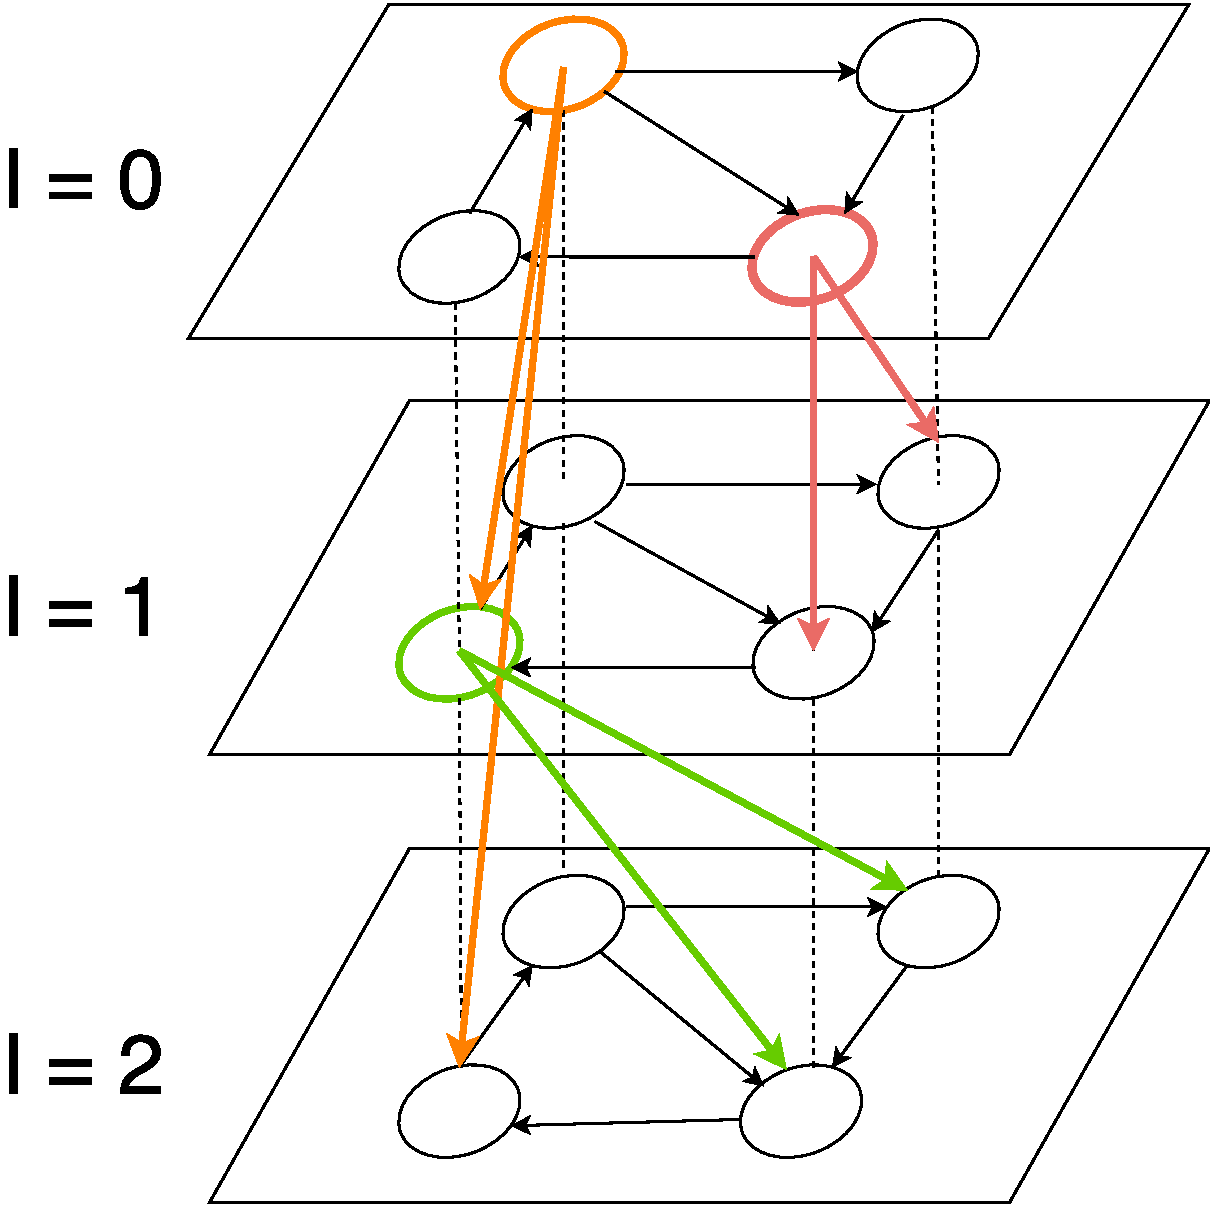
\includegraphics[scale=0.2]{nettowaku.pdf}
\caption{時空間ネットワーク}
\vspace{-2mm}
\label{nettowaku}
\end{figure}

馬谷の研究 \cite{馬谷さん卒論},また本研究では,地下空間の広がりと時間の
経過を同時に表現する時空間ネットワークを用いて最適化モデルを構築している.

時空間ネットワークは複数のレイヤを持つ.一つのレイヤ内に注目したとき,そ
の上には考察対象の空間を表すグラフが存在する.さらにこれらを重なることで,
時間経過を表現する.空間内の移動は時間経過を伴うから,単一レイヤ内でのフ
ローとしては表現するのではなく,レイヤ間のフローとして表現することになる.

%時空間ネットワークとは,空間の形状を表すネットワークに時間軸を加えて拡張
%したネットワークである.すなわち時空間ネットワーク上では場所と時間が同時
%に表現できるため,最初に出発する場所と経路から,目的となる場所と時刻まで
%の移動経路がリンクをたどることで求められる.図\ref{nettowaku}は地下街を想
%定したネットワークを表している.

本研究では,止水板を設置する各チームの移動回数を $l = 0, 1, 2, \ldots$ と
したとき,これを時空間ネットワークにおけるレイヤに対応させることで,設置
チームの移動を表現している.

%図\ref{nettowaku}では,止水板を設置する各チームの移動回数を $l = 0, 1,
%2,...$ とし,これを時空間ネットワークにおけるレイヤに対応させる.

%%%%%%%%%%%%%%%%%%%%%%%%%%%%%%%%%%%%%%%%%%%%%%%%%%%%%%%%%%%%%%%%%%%%%%
\vspace{-4mm}
\section{本研究で用いる最適化モデル}
\vspace{-2mm}

本研究で用いる最適化モデルは,\cite{馬谷さん卒論} で提案された問題に一部
修正,追加を行ったものである(表 \ref{制約条件表}).以下,最適化モデル
の目的関数と制約条件について説明する.
%
\vspace{-3mm}
\begin{table}[htpb]
  \begin{center}
    \caption{先行研究\cite{馬谷さん卒論}からの制約条件の訂正と追加}
    \begin{tabular}{ll}\hline
      \cite{馬谷さん卒論}で提案された制約 & 制約条件 $1~7$, $9$, $10$  \\
      \cite{馬谷さん卒論}で提案された制約を修正 & 制約条件 $8$  \\
      新たに追加する制約 & 制約条件 $11$  \\\hline
    \end{tabular}
    \label{制約条件表}
  \end{center}
\end{table}

\vspace{-8mm}
\begin{description}
 \item [目的関数] 流入開始時刻に間に合わなかった出入口の止水板設置完了時
	     刻と流入開始時刻の差($=$ 流入時間)の合計を最小化
	     \vspace{-2mm}
 \item [制約条件 1] 初期状態では,設置チームは定められたスタート地点に位
	     置している
	     \vspace{-2mm}
 \item [制約条件 2] 全出入口にはいずれかの設置チームが訪問し,全出入口に
	     止水板を設置する
	     \vspace{-2mm}
 \item [制約条件 3] 各設置チームはそれぞれの移動の際に高々 1 つの出入口に
	     位置することができる
	     \vspace{-2mm}
 \item [制約条件 4] 1 つの出入り口に移動するのは,いずれかの 1 チームのみ
	     である
	     \vspace{-2mm}
 \item [制約条件 5~7] 時空間ネットワークにおける枝と接点の関係性
	     \vspace{-2mm}
 \item [制約条件 8] 各出入り口の止水板設置完了時刻の計算
	     \vspace{-2mm}
 \item [制約条件 9] 流入開始するまでの時間の設定
	     \vspace{-2mm}
 \item [制約条件 10] 止水板設置完了時刻と流入開始時刻の差の計算
	     \vspace{-2mm}
 \item [制約条件 11] 各設置チームの稼働時間の制限
\end{description}

%%%%%%%%%%%%%%%%%%%%%%%%%%%%%%%%%%%%%%%%%%%%%%%%%%%%%%%%%%%%%%%%%%%%%%

%%%%%%%%%%%%%%%%%%%%%%%%%%%%%%%%%%%%%%%%%%%%%%%%%%%%%%%%%%%%%%%%%%%%%%
\section{数値実験}
\vspace{-2mm}
\subsection{計算環境と実験内容}
\vspace{-3mm}
%%%%%%%%%%%%%%%%%%%%%%%%%%%%%%%%%%%%%%%%%%%%%%%%%%%%%%%%%%%%%%%%%%%%%%

本実験で用いた計算環境は以下の通りである:
%
\vspace{-2mm}
%
\begin{itemize}
 \setlength{\parskip}{0cm} % 段落間
 \setlength{\itemsep}{0cm} % 項目間
 \item OS: Microsoft Windows 10 Home
 \item CPU: Intel(R) Core i7-6600U CPU @ 2.60GHz 2.81GHz
 \item メモリ:16.0GB
 \item ソルバ:Gurobi Optimizer
\end{itemize}
%\vspace{-8mm}
%\begin{figure}[htpb]
% \begin{center}
%  
\includegraphics[scale=0.3]{./KU.eps}
%  \caption{図や写真等のタイトルは下に配置}
%  \label{fig:1}
% \end{center}
%\end{figure}

また実験の基本設定は表 \ref{tb:ex1} の通りである.
本研究では以下の実験を行った.
%
\vspace{-2mm}
%
\begin{itemize}
 \setlength{\parskip}{0cm} % 段落間
 \setlength{\itemsep}{0cm} % 項目間
 \item 実験 1: 止水板の設置に必要な設置チーム数の算出
%       \begin{itemize}
%	\item 止水板設置チームの稼働時間に上限がある状況下で,越水する(で
%	      あろう)全ての出入り口に止水板を設置するために必要な設置チー
%	      ム数を算出する.
%       \end{itemize}
 \item 実験 2: 設置開始時刻と流入時間の合計の関係(稼働時間に上限がある場合)
%       \begin{itemize}
%	\item 設置開始時刻が遅くなれば,各出入り口からの流入時間の合計は
%	      大きくなるが,この関係を定量的に評価する.
%       \end{itemize}
 \item 実験 3: 設置チーム数と流入時間の合計の関係(稼働時間に上限がない場合)
%       \begin{itemize}
%	\item 稼働時間に上限がない場合,設置チーム数が少なくとも全ての出
%	      入り口に止水板を設置することができるが,流入時間の合計は大
%	      きくなるはずである.この関係を定量的に評価する.
%       \end{itemize}
\end{itemize}

\vspace{-5mm}
\begin{table}[htpb]
  \begin{center}
    \caption{数値実験の基本設定}
   \scalebox{0.8}{
    \begin{tabular}{ll}
      \hline
      計算対象地域 & ホワイティうめだ \\
      1 時間当たりの降雨量 & 120mm \\
      排水用ポンプ & 稼動状態 \\
      雨水が流入する出入り口の数 & 21 箇所 \\
%      止水板設置チーム数 & 2 $~$ 6 チーム \\
      止水板設置チームの歩行速度 & 66 m/分 \\
%      降雨開始から止水板設置開始までの時間 & 64 分 \\
      止水板 1 箇所の世知に要する時間 & 5 分 \\
%      スタート地点のメッシュ番号 & 15728 \\
%      1 チームの稼働時間の制限 & 30 分 \\
      \hline
    \end{tabular}
   }
    \label{tb:ex1}
  \end{center}
\end{table}

\vspace{-8mm}
\subsection{実験 1}

\vspace{-3mm}
本節では,止水板設置チームの稼働時間に上限がある状況下で,越水するとされ
る全ての出入り口に止水板を設置するために必要な設置チーム数を算出する.こ
こでは,以下の条件で計算を行う:
%
\vspace{-2mm}
%
\begin{itemize}
 \setlength{\parskip}{0cm} % 段落間
 \setlength{\itemsep}{0cm} % 項目間
 \item 止水板設置開始時刻: 64 分
 \item 設置チーム数: 2, 3, 4, 5, 6 チーム
 \item 設置チームの稼働時間の上限: 30, 40, 50, 60 分
\end{itemize}
%
\vspace{-2mm}
%
ここで,止水板設置開始時刻の 64 分とは,想定する豪雨(120mm/hr)が降り始
めてから,ホワイティうめだの出入り口で最初に越水が始まるとされる時刻であ
る.

\vspace{-5mm}
\begin{table}[htpb]
 \begin{center}
  \caption{止水板の設置可能性}
  \scalebox{0.8}{
  \begin{tabular}{c|cccc}\hline
            & \multicolumn{4}{c}{稼働時間} \\ 
   チーム数 & 30 & 40 & 50 & 60\\\hline
   6 & 可能 & 可能 & 可能 & 可能\\
   5 & 暫定解なし & 可能 & 可能 & 可能\\
   4 & 不可能 & 可能 & 可能 & 可能\\
   3 & 不可能 & 不可能 & 暫定解なし & 可能\\
   2 & 不可能 & 不可能 & 不可能 & 不可能\\\hline
  \end{tabular}
  }
  \label{64分制限時間変化}
 \end{center}
\end{table}

\vspace{-5mm}
%
計算結果を表 \ref{64分制限時間変化} に示す.表 \ref{64分制限時間変化} で
の「暫定解なし」となっているのは,最適化計算によって,所定の時間(3600 秒)
内に暫定解を得ることができず,設置が可能であるかどうかが判定できないこと
を表す.

本実験から,設置チーム数が $6$ のときは,稼働時間の上限が(最短の)$30$
分であっても,越水する全て出入り口に止水板を設置可能であることがわかった.

\vspace{-3mm}
\subsection{実験 2}

\vspace{-3mm}
%
設置開始時刻が遅くなれば,各出入り口からの流入時間の合計は大きくなるはず
である.ここでは,この関係を定量的に評価するために,以下の条件で計算を行
う:
%
\vspace{-2mm}
%
\begin{itemize}
 \setlength{\parskip}{0cm} % 段落間
 \setlength{\itemsep}{0cm} % 項目間
 \item 止水板設置開始時刻: 43, 57, 64 分
 \item 設置チーム数: 6 チーム
 \item 設置チームの稼働時間の上限: 30 分
\end{itemize}
%
\vspace{-2mm}
%
ここで,止水板設置開始時刻の 43, 57, 64 分は,ホワイティうめだにおいて
「水位計より判断」した時間,「地上監視カメラより判断」した時間,「地下へ
の流入が始まった」時間に対応している.

\vspace{-2mm}
\begin{table}[htpb]
  \begin{center}
   \caption{設置開始時刻と流入時間の合計の関係}
   \scalebox{0.8}{
   \begin{tabular}{cc}\hline
     設置開始時刻(分) & 流入時間の合計 (分) \\
     \hline
     43 & 0.00 \\
     57 & 6.03 \\
     64 & 13.91 \\
     \hline
   \end{tabular}
   }
   \label{tb:ex2}
  \end{center}
\end{table}

\begin{figure}[htpb]
 \begin{center}
  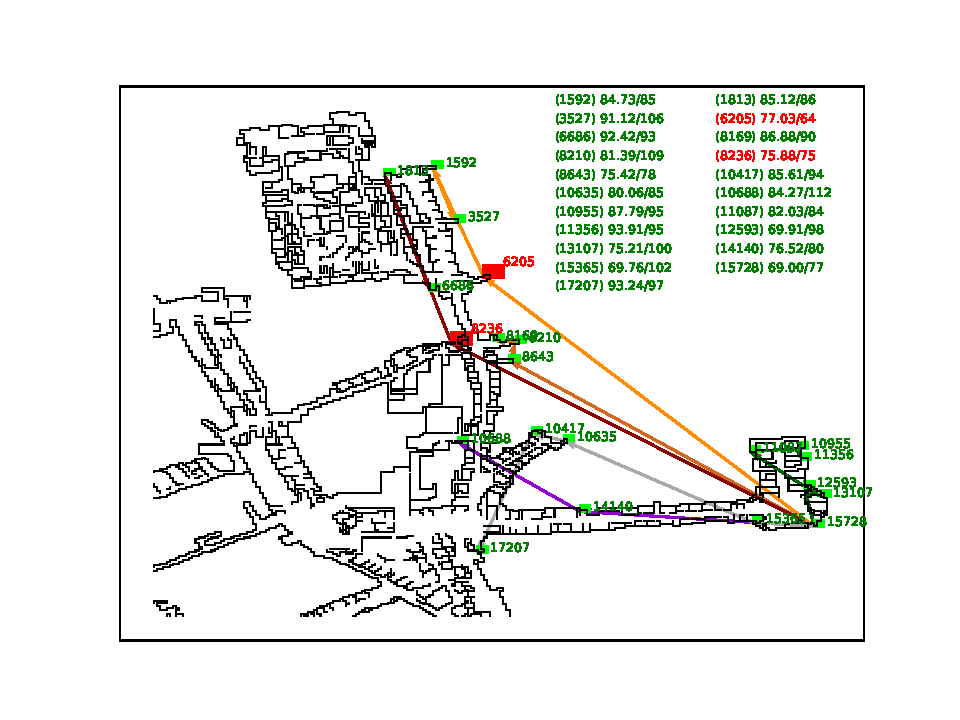
\includegraphics[width=3.5cm,trim=100 50 100 50]{../fig/64min_6team_lim30min.pdf}
  \caption{設置開始時刻 64 分での最
  適な止水板設置順序}
  \label{fig:64min_6team_lim30min_}
 \end{center}
\end{figure}

\vspace{-5mm}
計算結果を表 \ref{tb:ex2} に示す.設置開始時刻が遅くなるにつれ,流入時間
の合計が大きくなることを定量的に算出できている.
%
また設置開始時刻が $64$ 分の場合の最適な設置経路を図
\ref{fig:64min_6team_lim30min_} に示す.

\vspace{-3mm}
\subsection{実験 3}

\vspace{-3mm}
稼働時間に上限がない場合,設置チーム数が少なくとも全ての出入り口に止水板
を設置することができるが,流入時間の合計は大きくなるはずである.本節では,
この関係を定量的に評価するために,以下の条件で計算を行う:
%
\begin{itemize}
 \setlength{\parskip}{0cm} % 段落間
 \setlength{\itemsep}{0cm} % 項目間
 \item 止水板設置開始時刻: 43, 57, 64 分
 \item 設置チーム数: 2, 3, 4, 5, 6 チーム
 \item 設置チームの稼働時間の上限: なし
\end{itemize}

%止水板設置開始時刻と設置チーム数の変化に伴って,流入時間の合計がどのよう
%に変化するかをまとめたものが表 \ref{tb:ex3} である.

\vspace{-5mm}
%
\begin{table}[htpb]
 \begin{center}
  \caption{チーム数・設置開始時刻と流入時間の合計の関係}
  \scalebox{0.8}{
  \begin{tabular}{c|ccc}
   \hline
   & \multicolumn{3}{c}{止水板設置開始時刻} \\
   設置チーム数 & 43 & 57 & 64 \\
   \hline
   6 & 0.00  & 6.03   & 13.91 \\
   5 & 0.00  & 6.03   & 13.91 \\
   4 & 0.00  & 6.03   & 24.21 \\
   3 & 0.00  & 34.73  & 138.82 \\
   2 & 66.76 & 203.70 & 288.33 \\
   \hline
  \end{tabular}
  }
  \label{tb:ex3}
 \end{center}
\end{table}

\vspace{-3mm}
表 \ref{tb:ex3} からわかるように,
%いずれの設置開始時刻の場合も,
設置チーム数が少なくなるにつれて,流入時間の合計が急激に増加する.すなわ
ち,防災・減災の観点からは,一定以上の設置チーム数を確保しておくことが必
須である.
%
しかしながら,例えば夜間などのことを想定すると,設置チーム数が潤沢に準備
できない状況も想定される.そのような場合には,本計算で得られた最適な設置
順序を用いることによって,被害を最小限に食い止めることができるであろう.

\begin{comment}

%%%%%%%%%%%%%%%%%%%%%%%%%%%%%%%%%%%%%%%%%%%%%%%%%%%%%%%%%%%%%%%%%%%%%%
\subsection{実験 1}
\vspace{-2mm}
%%%%%%%%%%%%%%%%%%%%%%%%%%%%%%%%%%%%%%%%%%%%%%%%%%%%%%%%%%%%%%%%%%%%%%

実験 1 では,以下の条件で計算を行った:
\vspace{-3mm}
\begin{table}[H]
 \begin{center}
   \caption{実験 1 で設定した条件}
  \begin{tabular}{ll}
   \hline
   1 時間あたりの降雨量 & 120mm \\
   排水用ポンプ & 稼働 \\
   雨水が流入する出入口の数 & 21 箇所 \\
   止水板設置チーム数 & 2~6 チーム \\
   止水板設置チームの歩行速度 & 66 m/分  \\
   降雨開始から止水板設置開始までの時間 & 64分 \\
   止水板 1 箇所の設置に要する時間 & 5 分 \\
   1 チームの稼働時間の制限 & 30 分\\
   \hline
  \end{tabular}
  \label{tb:ex1}
 \end{center}
\end{table}
\vspace{-6mm}
本研究では,梅田地下街全域ではなくホワイティうめだに限定して最適設置順序を算出する.図\ref{ホワイティ}は 1 時間あたりの降雨量が 120 mm のとき,排水用ポンプが稼働しているときに雨水が流入すると推定されるホワイティ梅田に存在する地下街出入り口である.本実験では,これらに対し,2~6 チームで止水板の設置を行うことを想定する.降雨開始直後では地下に雨水が流入しないので,本実験では止水板設置開始時刻を 64,57,43 分と想定する.なお,大阪地下街防災センターの近くにある出入り口をスタート地点としている.
\begin{figure}[H]
  \centering
  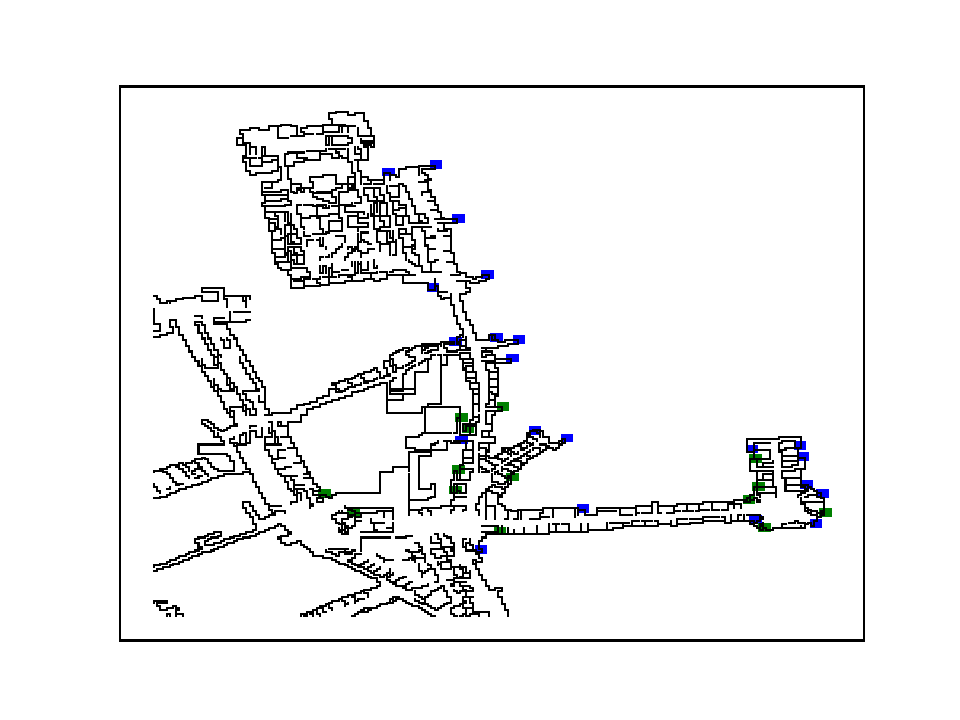
\includegraphics[width=80mm]{whity_map.pdf}
  \vspace{-4mm}
  \caption{ホワイティうめだ 出入口図}
  \label{ホワイティ}
\end{figure}


%% \begin{figure}[H]
%%   \begin{tabular}{cc}
%%   \begin{minipage}{0.5\hsize}
%%   \begin{center}
%%     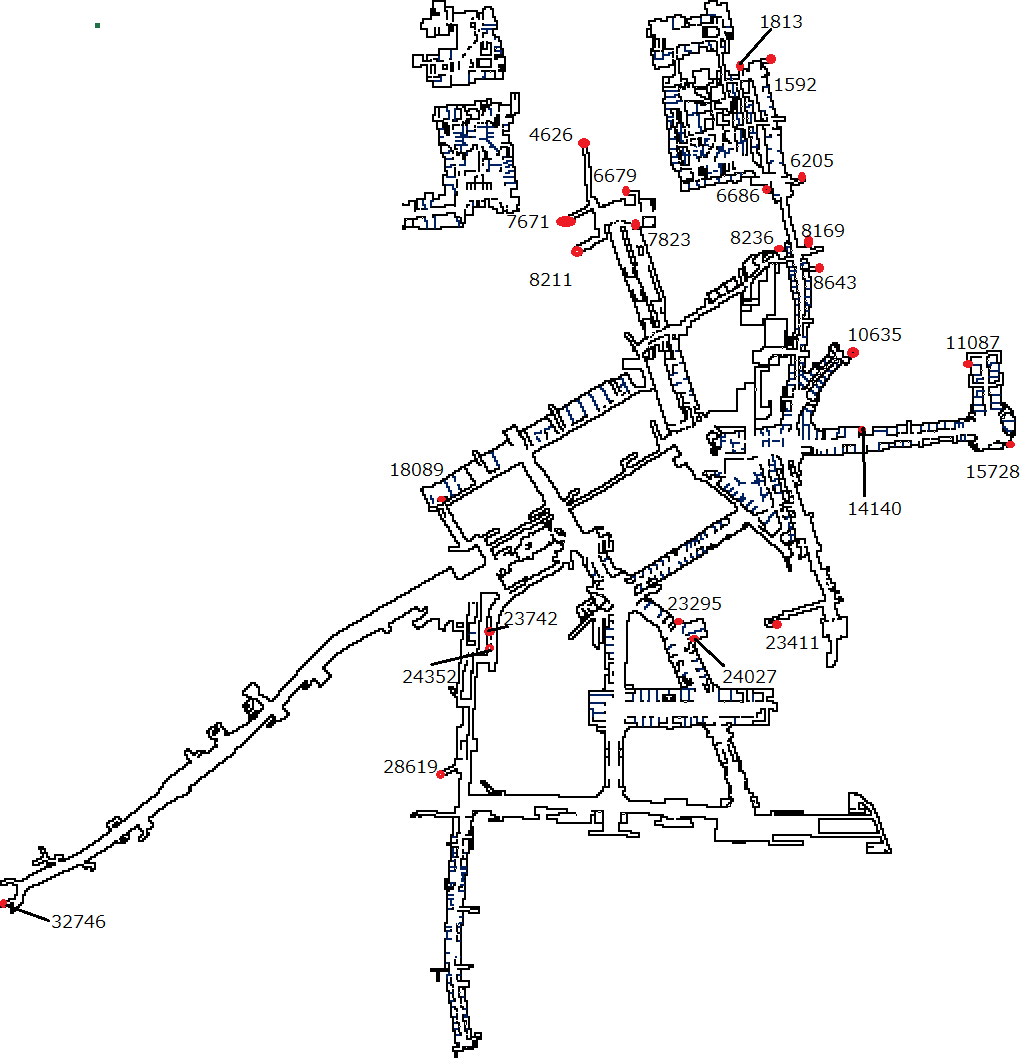
\includegraphics[width=30mm]{umedamap.png}
%%   \end{center}
%%   \vspace{-5.2mm}
%% \caption{出入口流入箇所}
%% \label{fig:zikken2_4team_gurahu}
%% \end{minipage}
%% \begin{minipage}{0.5\hsize}
%% \begin{center}
%% 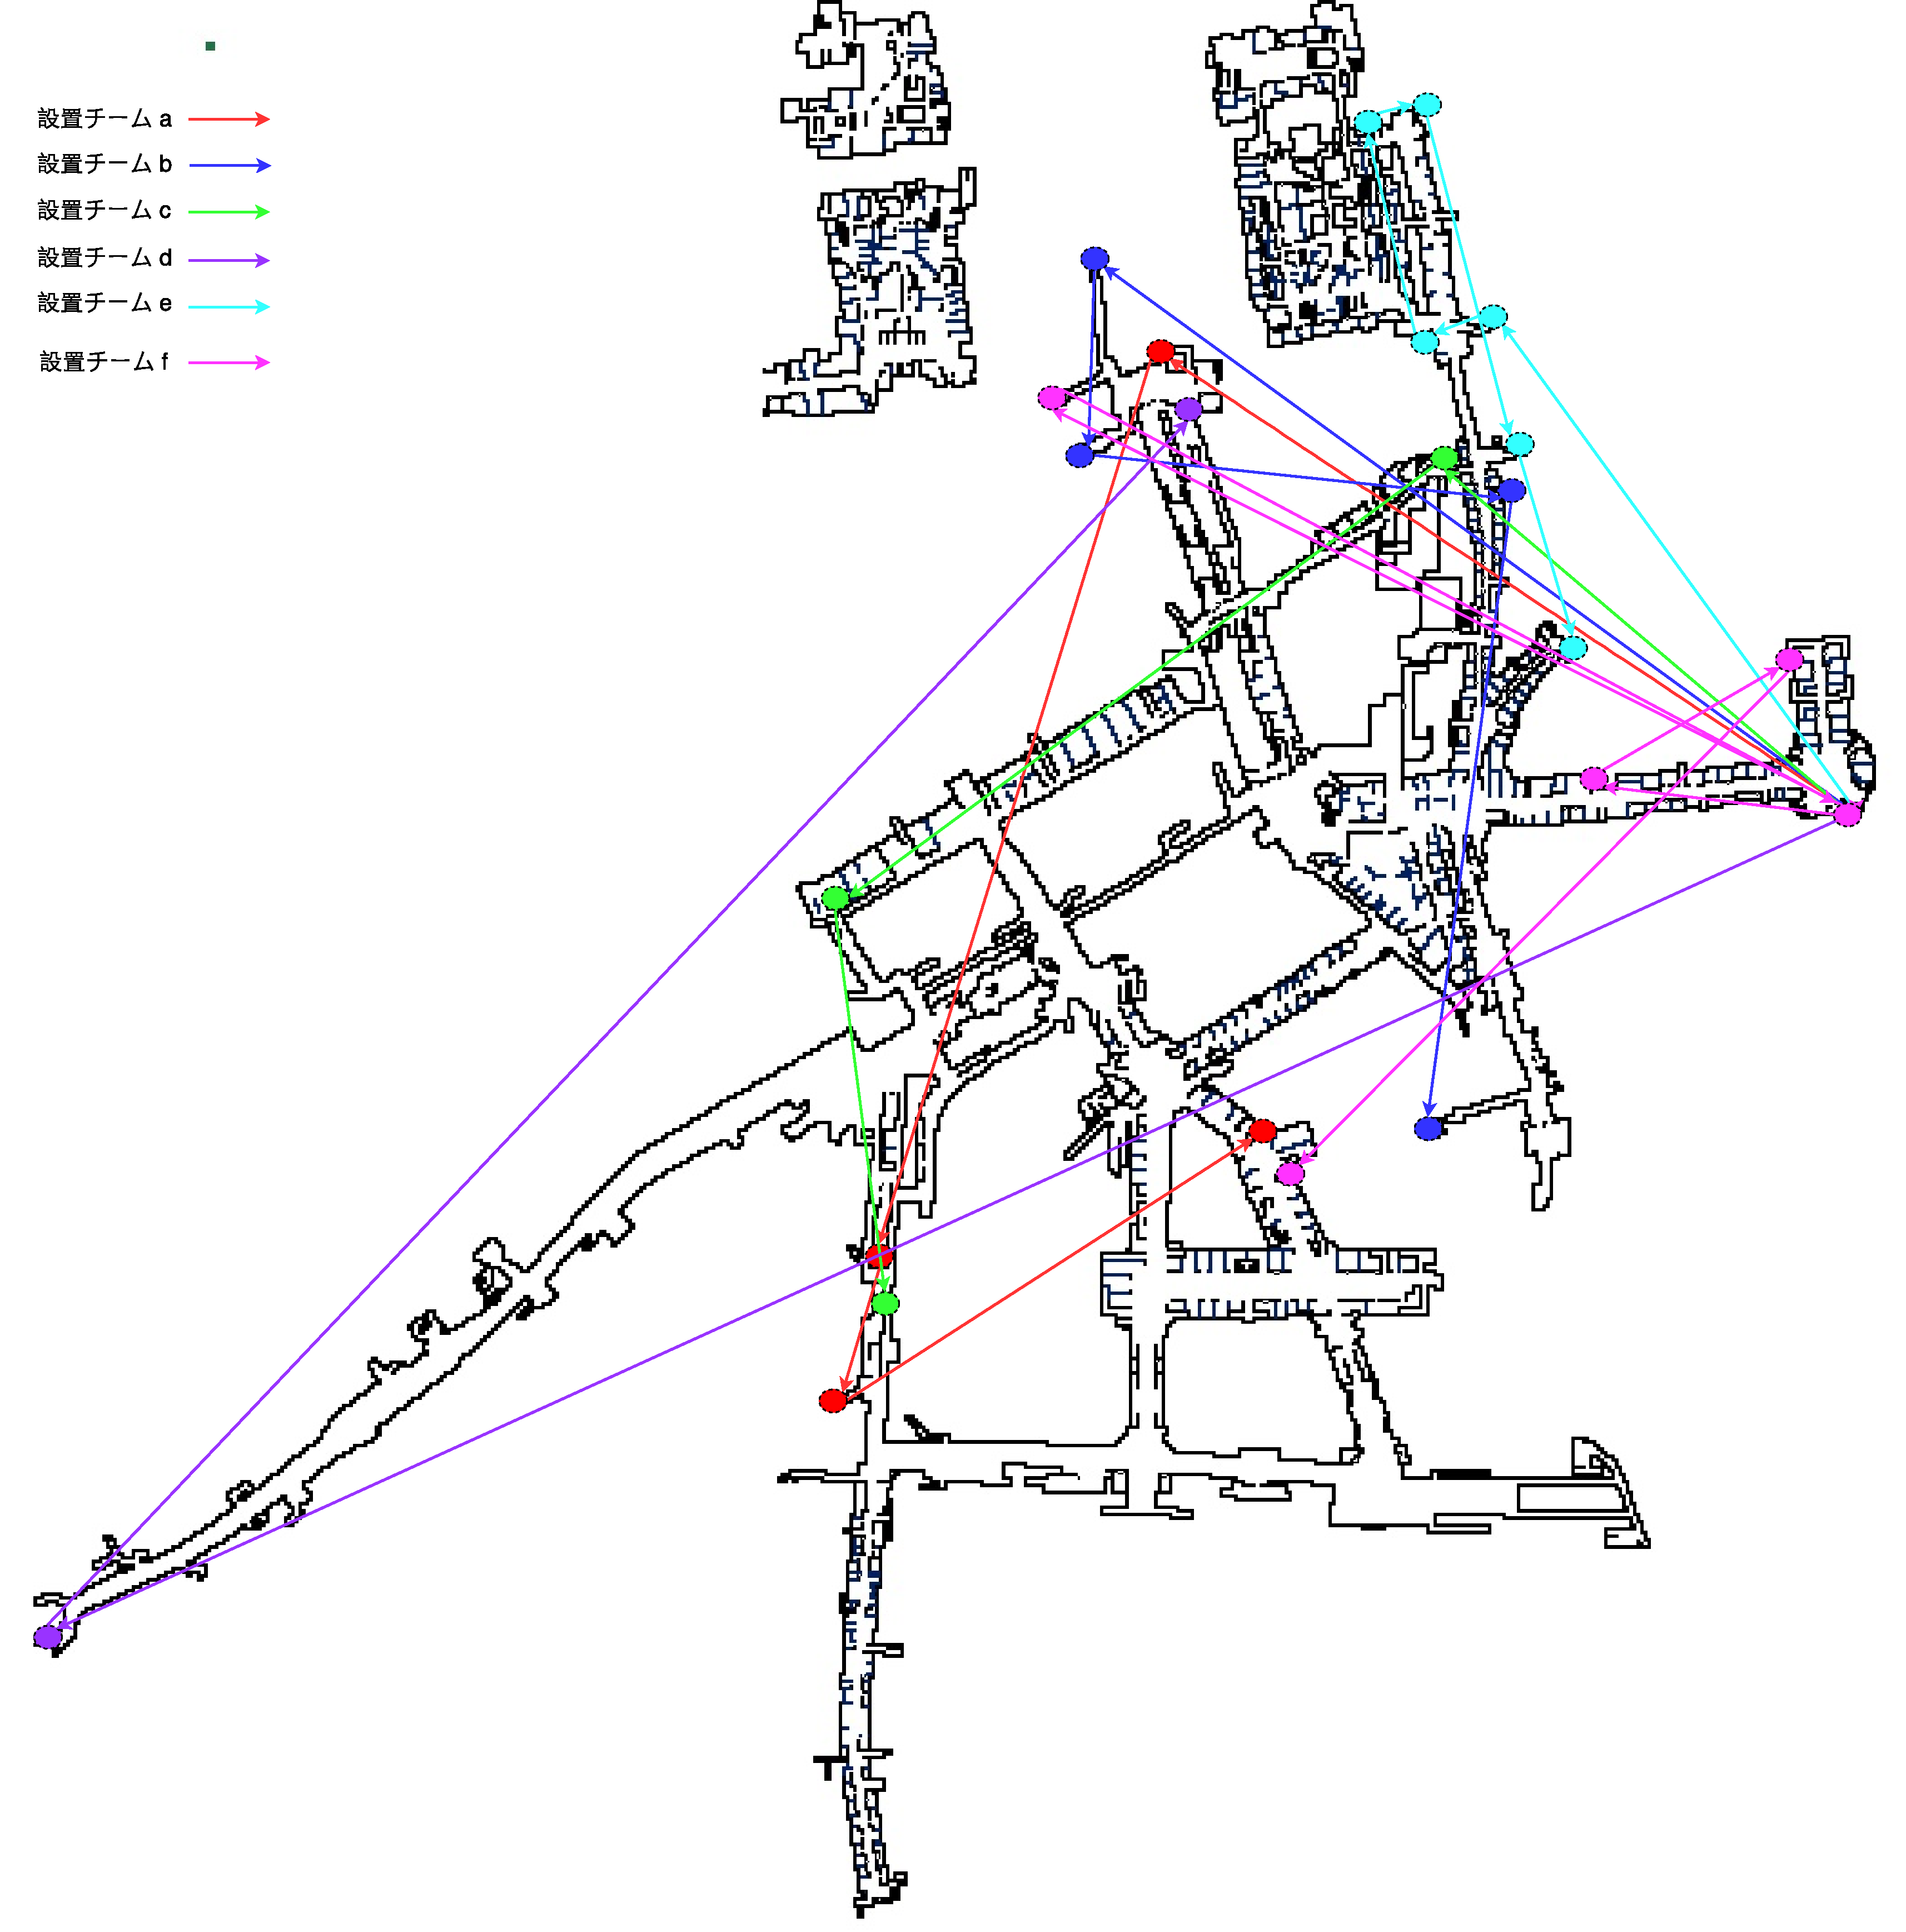
\includegraphics[width=30mm]{zikken1_settizyunzyo_map.pdf}
%% \end{center}
%% \vspace{-5.2mm}
%% \caption{最適設置順序 (実験 1)}
%% \label{fig:zikken2_5team_gurahu}
%% \end{minipage}
%% \end{tabular}
%% \end{figure}
%% \vspace{-4mm}
%% \begin{figure}[H]
%% \centering
%% 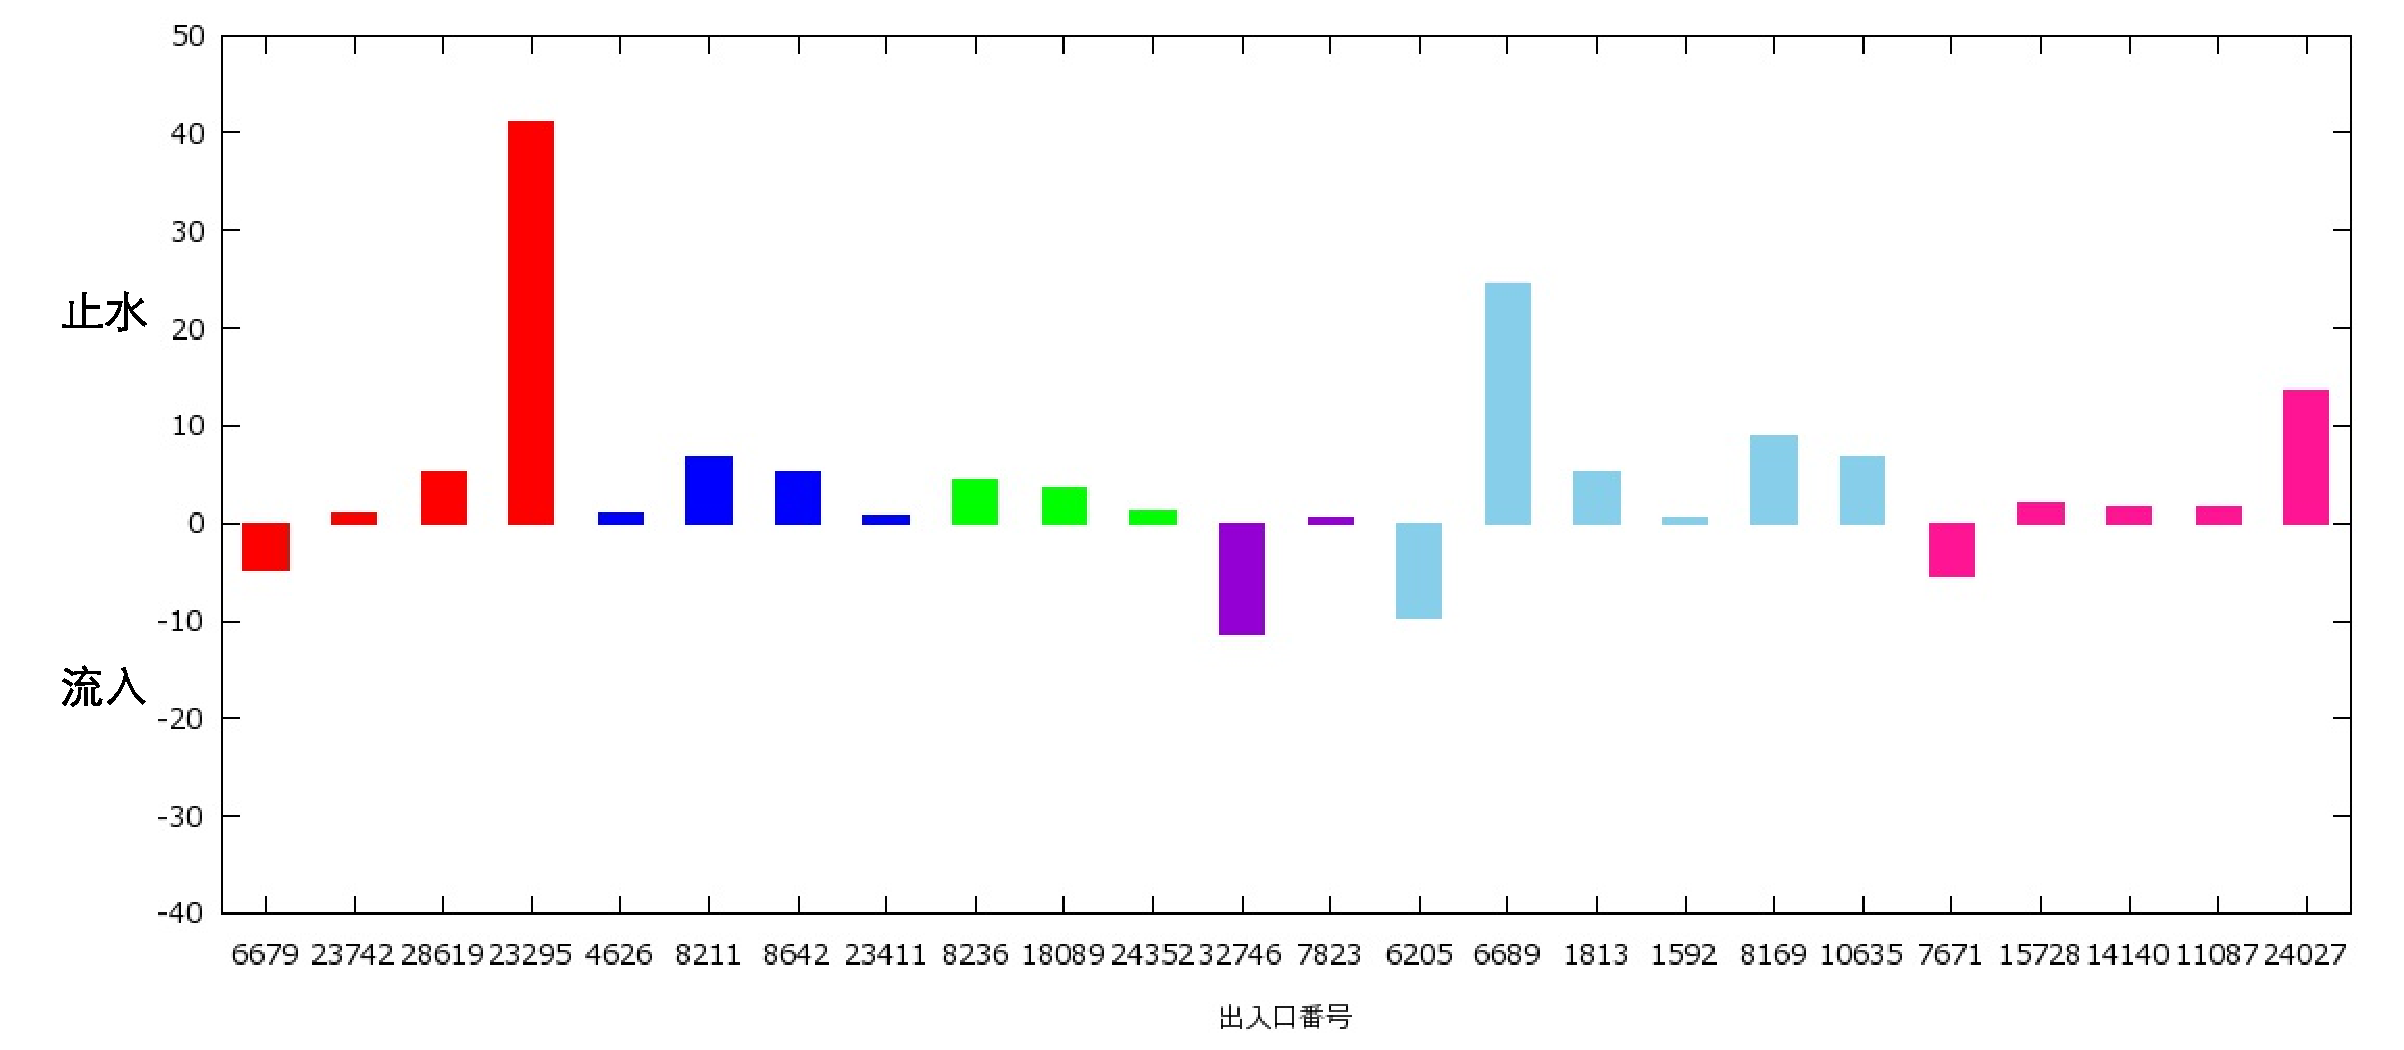
\includegraphics[scale=0.2]{zikken1_gurahu}
%% \vspace{-4mm}
%% \caption{梅田地下街 流入状況 }
%% \label{fig:zikken1_gurahu}
%% \end{figure}

\begin{table}[H]
\begin{center}
\caption{稼働時間 30 分の流入時間}
\begin{tabular}{l|ccc}\hline
\backslashbox{($A$)}{($B$)} & 64 & 57 & 43\\\hline
6 & 13.91 & 6.0 & 0.0\\     
5 & 暫定解なし & 暫定解なし & 暫定解なし\\
4 & 実行不可能 & 実行不可能 & 実行不可能\\
3 & 実行不可能 & 実行不可能 & 実行不可能\\
2 & 実行不可能 & 実行不可能 & 実行不可能\\\hline
\end{tabular}
\label{30分制限あり}
\end{center}
\end{table}

\begin{table}[H]
\begin{center}
\caption{稼働時間上限なしの流入時間}
\begin{tabular}{l|ccc}\hline
\backslashbox{($A$)}{($B$)} & 64 & 57 & 43\\\hline
6 & 13.91 & 6.03 & 0.00\\
5 & 13.91 & 6.03 & 0.00\\
4 & 24.21 & 6.03 & 0.00\\
3 & 138.82 & 34.73 & 0.00\\
2 & 288.33 & 203.70 & 66.76\\\hline
\end{tabular}
\label{30分制限なし}
\end{center}
\end{table}

\hspace{2.0cm}($A$) : 設置チーム数\\
\hspace{2.4cm}($B$) : 止水板設置開始時刻(分)\\
\vspace{-4mm}

表\ref{30分制限あり},表\ref{30分制限なし} は止水板設置開始 64~43 分に変化させた時に設置チームを 2~6 チームの場合で計算した結果の流入時間を表している.この結果から設置チーム 4~6 チームでは流入時間に大きな変化見られないが, 2 チームまで少なくなると,流入時間は大幅に長くなることが分かる.止水板設置開始時刻による流入時間の差もチーム数が少なくなるごとに大きくなっている.

\vspace{-4mm}
%%%%%%%%%%%%%%%%%%%%%%%%%%%%%%%%%%%%%%%%%%%%%%%%%%%%%%%
\subsection{実験 2}
\vspace{-2mm}
%%%%%%%%%%%%%%%%%%%%%%%%%%%%%%%%%%%%%%%%%%%%%%%%%%%%%%%%%%%%%%%%%%%%%%
 実験 2 では,各設置チームの稼働時間を 40~60 分に変化させて流入するすべての出入り口に止水板設置可能か検討した.
\vspace{-4mm}

\begin{table}[H]
\begin{center}
  \caption{実験 $2$ : 計算結果}
  \scalebox{0.8}{
\begin{tabular}{l|cccc}\hline
\backslashbox{チーム数}{稼働時間} & 30 & 40 & 50 & 60\\\hline
6 & 可能 & 可能 & 可能 & 可能\\
5 & 暫定解なし & 可能 & 可能 & 可能\\
4 & 不可能 & 可能 & 可能 & 可能\\
3 & 不可能 & 不可能 & 暫定解なし & 不可能\\
2 & 不可能 & 不可能 & 不可能 & 不可能\\\hline
\end{tabular} }
\label{64分制限時間変化}
\end{center}
\end{table}

表\ref{64分制限時間変化} は止水板設置可能であるかを示した表である.4,5 チームの場合では,稼働時間を 40 分にすると設置が可能になる.3,2 チームは制限時間を設けると制限時間内に全ての止水板設置することは不可能であることが分かった.\\
%%%%%%%%%%%%%%%%%%%%%%%%%%%%%%%%%%%%%%%%%%%%%%%%%%%%%%%%%%%%%%%%%%%%%%%%%%%%%%%%%%%%%%%%%%%%%%%%%%%%
\subsection{実験 3}
\vspace{-2mm}
%%%%%%%%%%%%%%%%%%%%%%%%%%%%%%%%%%%%%%%%%%%%%%%%%%%%%%%%%%%%%%%%%%%%%%%%%%%%%%%
実験 3 では,実験 1 で算出した止水板設置開始時刻 64 分の場合の設置経路に固定して,設置開始時刻を 57,43 分に変化させたとき,流入時間に差は出るのかを比較した.
\begin{table}[H]
\begin{center}
  \caption{実験 $3$: 計算結果}
  \scalebox{0.8}{
\begin{tabular}{l|ccc}\hline
\backslashbox{チーム数}{} & 設置開始時刻 & 稼働時間 & 流入時間の合計(分)\\\hline
6 & 57 & 30 & 6.03\\
6 & 57 & $-$ & 6.03\\
5 & 57 & $-$ & 6.03\\
4 & 57 & $-$ & 6.03\\
6 & 43 & 30 & 0.00\\
6 & 43 & $-$ & 0.00\\
5 & 43 & $-$ & 0.00\\
4 & 43 & $-$ & 0.00\\\hline
\end{tabular} }
\label{経路固定_止水板設置開始57分}
\end{center}
\end{table}

この結果より,経路を固定して止水板設置開始時刻を変化させても流入時間に変化はなかった.つまり,設置開始時刻によって設置順序を変える必要がないことが分かった.\\
\vspace{-5mm}

\end{comment}

%%%%%%%%%%%%%%%%%%%%%%%%%%%%%%%%%%%
%\section{おわりに}
%%%%%%%%%%%%%%%%%%%%%%%%%%%%%%%%%%%%%%%%%%%%%%%%%%%%%%%%%%%%%%%%%%%%%

%%%%%%%%%%%%%%%%%%%%%%%%%%%%%%%%%%%%%%%%%%%%%%%%%%%%%%%%%%%%%%%%%%%%%
% 数式は,\verb|align| 環境を用いて入力すること.
%
%\begin{align}
% G &= \sum_{n = 0}^\infty b_n(t)
% \label{eq:G} \\
% F &= \int_\Gamma \sin z \; {\rm d}z
% \label{eq:F}
%\end{align}
%
%%%%%%%%%%%%%%%%%%%%%%%%%%%%%% 
%%%%%%%%%%%%%%%%%%%%%%%%%%%%%%
\begin{comment}

\begin{table}
 \begin{center}
  \caption{表のタイトルは上に配置}
  \begin{tabular}{|l|l|l|}
   \hline
   A \hspace{2cm} & B \hspace{2cm} & C \hspace{2cm} \\
   \hline
   あ & い & う \\
   \hline
  \end{tabular}
  \label{tb:1}
 \end{center}
\end{table}

\end{comment}
%%%%%%%%%%%%%%%%%%%%%%%%%%%%%%%%%%%%%%%%%%%%%%%%%%%%%%%%%%%%%%%%%%%%%%
%%%%%%%%%%%%%%%%%%%%%%%%%%%%%%%%%%%%%%%%%%%%%%%%%%%%%%%%%%%%%%%%%%%%%%
\begin{comment}
文献や式・図表の引用は以下のように:
\begin{itemize}
 \item \cite{都市12}
 \item 式 (\ref{eq:G})
 \item 図 \ref{fig:1}
 \item 表 \ref{tb:1}
\end{itemize}
\end{comment}

%%%%%%%%%%%%%%%%%%%%%%%%%%%%%%%%%%%%%%%%%%%%%%%%%%%%%%%%%%%%%%%%%%%%%
\vspace{-3mm}
\section{おわりに}

\vspace{-3mm}
%
本研究では,\cite{馬谷さん卒論} で提案された最適化問題を改良しつつ,設置
者の稼働時間や地下街の管理区分を考慮しながら,最適な止水板の設置順序を算
出した.

現在用いている最適化モデルでは,表 \ref{64分制限時間変化} でもあったよう
に,一定の計算時間を確保しても暫定解が得られないなど,計算時間が長くなる
傾向がある.これを改良することが今後の課題である.

%%%%%%%%%%%%%%%%%%%%%%%%%%%%%%%%%%%%%%%%%%%%%%%%%%%%%%%%%%%%%%%%%%%%%
{\footnotesize
\begin{thebibliography}{9}
 \setlength{\parskip}{0cm} % 段落間
 \setlength{\itemsep}{0cm} % 項目間
 \bibitem{水工学論文集2}
	 %
	 井上知美,川中龍児,石垣泰輔,尾崎平,戸田圭一,
	 %
	 内水氾濫による大規模地下街の浸水過程と避難の安全性に関する検討,
	 %
	 水工学論文集,$55$, s$973$-s$978$ ($2011$).
 \bibitem{馬谷さん卒論}
	 %
	 馬谷慎太郎,
	 %
	 流入開始時刻を考慮した地下街出入口への最適な止水板設
	 置順序の算出,
	 %
	 関西大学環境都市工学部 $2016$ 年度卒業論文 ($2017$).
 \bibitem{武田さん卒論}
	 %
	 武田侑也,
	 %
	 大規模地下空間における内水氾濫による浸水対策の検討,
	 %
	 関西大学環境都市工学部 $2015$ 年度卒業論文 ($2016$).
 \bibitem{水工学論文集1}
	 %
	 森兼政行,石垣泰輔,尾崎平,戸田圭一,
	 %
	 大規模地下空間を有する都市域における地下空間への内水氾濫水の流入
	 特性とその対策,
	 %
	 水工学論文集 , $55$, s$967$-s$972$ ($2011$).
\end{thebibliography}
}
%%%%%%%%%%%%%%%%%%%%%%%%%%%%%%%%%%%%%%%%%%%%%%%%%%%%%%%%%%%%%%%%%%%%%%

\end{document}

%%%%% End of file %%%%%

